% FUSAO (26/10/2026): float copied unchanged from tables_C*.tex, tables_main.tex or tables_appendix.tex.
\begin{figure}[htbp]\centering
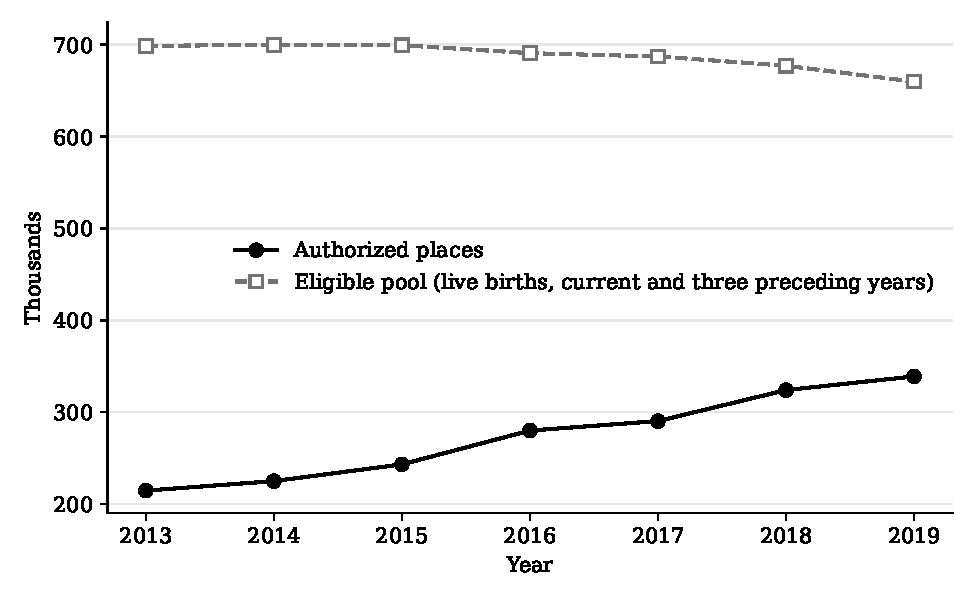
\includegraphics[width=0.85\textwidth]{F7_capacidade_pool}
\caption{Authorized childcare places in the first semester and the eligible population based on annual live births, S\~ao Paulo, 2013--2019}
\label{fig:F7}
\tabnote{\emph{Sources:} Municipal class profile (authorized places, first semester); SINASC live births. Authorized places refer to the first semester of each year. The eligible population is calculated as the sum of live births in the reference calendar year and the preceding three years. It is not scaled to Census counts and therefore differs from the population series in Table~\ref{tab:arms}. Both series are shown as descriptive levels, expressed in thousands.}
\par\smallskip\noindent\begin{minipage}{\linewidth}\footnotesize\raggedright Alt text: Line chart comparing two annual series, measured in thousands, from 2013 to 2019. One series shows authorized childcare places in the first semester of each year; the other shows the eligible population calculated from live births in that year and the three preceding years.\end{minipage}
\end{figure}
